\documentclass[10pt]{scrartcl}

\usepackage[utf8]{inputenc}
\usepackage{tabularx}
\usepackage{longtable}
\usepackage[ngerman]{babel}
\usepackage[automark]{scrpage2}
\usepackage{amsmath,amssymb,amstext}
%\usepackage{mathtools}
\usepackage[]{color}
\usepackage[]{enumerate}
\usepackage{graphicx}
\usepackage{lastpage}
\usepackage[perpage,para,symbol*]{footmisc}
\usepackage{listings} 
\usepackage[pdfborder={0 0 0},colorlinks=false]{hyperref}
\usepackage[numbers,square]{natbib}
\usepackage{color}
\usepackage{colortbl}
\usepackage[absolute]{textpos}
\usepackage{float}

\lstset{numbers=left, numberstyle=\tiny, numbersep=5pt, breaklines=true, showstringspaces=false} 
\restylefloat{figure}

%changehere
\def\titletext{Lab 1 : MANET}
\def\titletextshort{Praktikum 1}
\author{André Harms, Oliver Steenbuck}

\title{\titletext}

%changehere Datum der Übung
\date{09.11.2011}

\pagestyle{scrheadings}
%changehere
\ihead{TT1, Schmidt}
\ifoot{Generiert am:\\ \today}

\cfoot{Oliver Steenbuck, André Harms}


\ohead[]{\titletextshort}
\ofoot[]{{\thepage} / \pageref{LastPage}}

\setlength{\parindent}{0.0in}
\setlength{\parskip}{0.1in}

\begin{document}
\maketitle

\setcounter{tocdepth}{3}
\tableofcontents

	\listoftables                                 												% 
	\listoffigures   

\section{Testaufbau}
	Die vier im Test verwendeten Router (APs) (110, 210, 104, 204) wurden wir in Abbildung \ref{img:testAufbau} gezeigt angeordnet. 	Von allen Access Points wurden die Antennen entfernt um reale Umgebungsbedingungen im Labor zu simulieren und den Aufbau eines Mesh-Netzwerkes zu ermöglichen. Beispielhaft sind in den Listings \ref{code_110_babel} und \ref{code_110_olsr} die Konfiguration des Babel bzw. OLSR Daemons für den Router 110 dargestellt, mit Ausnahme der entsprechend geänderten Adressen wurden alle Router identisch konfiguriert.  
		Alle Messungen wurden mit JPerf zwischen an den Routern 204 und 110 angeschlossenen Workstations durchgeführt, die Anzahl der Hops die zwischen den Messpunkten wurden mit Tracert, bzw. über die Weboberfläche des OLSR Daemons festgestellt. Ziel des Versuchsaufbaus war es das Mesh-Netzwerk so aufzubauen das Messungen über alle 4 Router hinweg durchgeführt werden können.
		
	\begin{figure}[H]
        \centering
                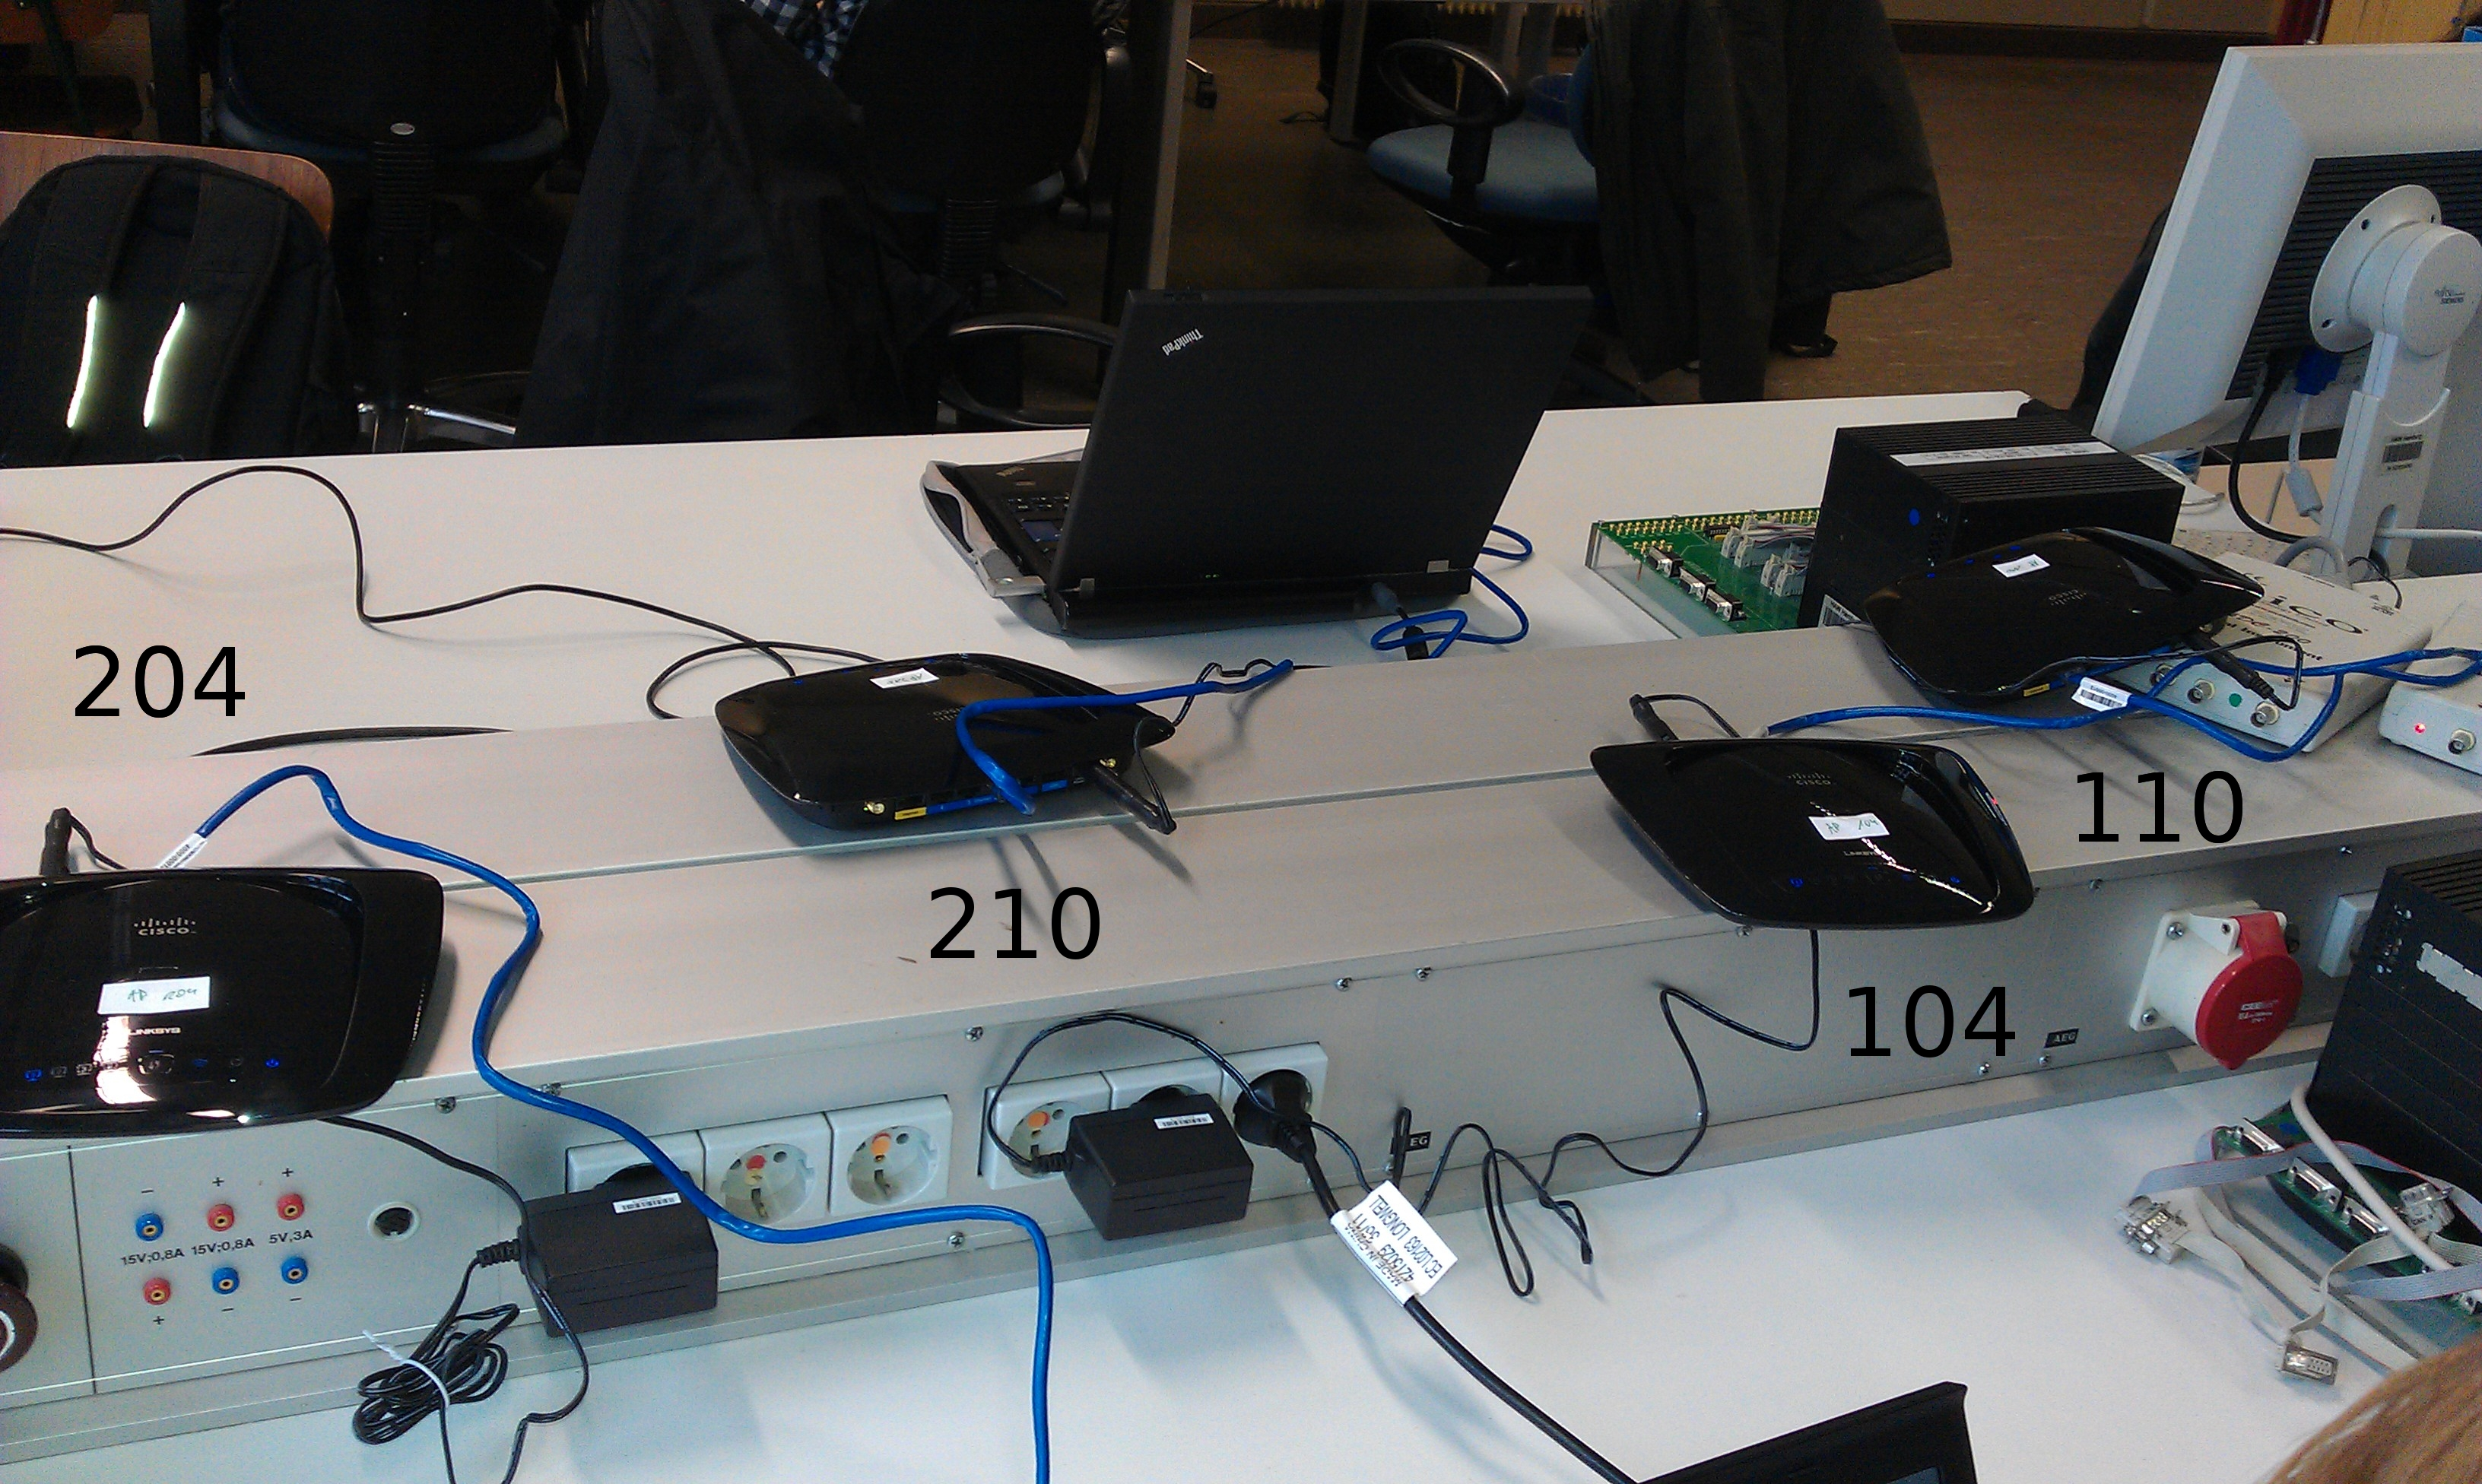
\includegraphics[width=\textwidth]{img/AufbauBild}
        \caption{Physikalische Anordnung Router}
        \label{img:testAufbau}
	\end{figure}	
	
	
	\lstinputlisting[label=code_110_babel,caption=Babel Konfiguration: Router 110, frame=single, language=bash]{../Startscripte/110/babeld_start.sh}	
	\lstinputlisting[label=code_110_olsr,caption=OLSR Konfiguration: Router 110, frame=single, language=bash]{../Startscripte/110/olsrd_start.sh}	
	
	
\section{Routing Protokolle}
	Im folgenden werden die beiden genutzen Routing Protokolle Babel und OLSR kurz erläutert und verglichen.
	
	\subsection{Babel}
	Bei Babel	
	
	
	\subsection{OLSR}

\section{Babel}
	\subsection{Experiment 1}
	Bei diesem Experiment wurden 10 MB mittels IPerf zwischen 2 Hosts ausgetauscht. Dabei wurde der Traffic über 3 Router geleitet (110-204-104) und UDP als Protokoll verwandt. Die TX-Power eines Routers (110) war dabei auf 11 gestellt alle anderen Geräte wurden mit TX-Power = 1 betrieben.
	
	\subsection{Experiment 2}
	Failover	
	
	\subsection{Experiment 3}
	Dieses Experiment wurde analog zu Experiment 1 durchgeführt, allerdings wurde diesmal die TX-Power bei allen Geräten auf 1 gesetzt.
	\begin{figure}[H]
        \centering
                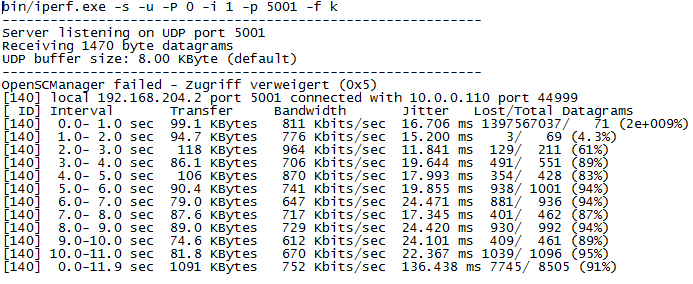
\includegraphics[width=\textwidth]{img/Babel_TX1_Protokoll}
        \caption{IPerf Log mit TX-Power=1}
        \label{img:babel_iperf_tx1}
	\end{figure}
	
	Im Kontrast zu Experiment 1, in dem einer der Router mit TX-Power=11 sendete, ist eine um 38\% Punkte höhere Paketverlustrate zu beobachten. Dieser Unterschied von gut einem Drittel resultiert aus der Tatsache, dass die Verbindung zwischen den beiden Routern 110 und 104 eine gleich schlechte Verbindung aufweist, und natürlich die Verbindung über 3 Geräte dadurch in seiner Gesamtheit leidet.

\section{OLRS}
	\subsection{Experiment 1}
	Traffic über 3 Hops	
	
	\subsection{Experiment 2}
	Failover, recovery nach neustart des abgebauten Routers


%\section{Anhang}
	%\subsection{Router Konfigurationen}
		%\lstinputlisting[label=code_110_babel,caption=Babel Konfiguration: Router 110, language=bash]{../Startscripte/110/babeld_start.sh}	
		%\lstinputlisting[label=code_110_olsr,caption=OLSR Konfiguration: Router 110, language=bash]{../Startscripte/110/olsrd_start.sh}	
		%\lstinputlisting[label=code_210_babel,caption=Babel Konfiguration: Router 210, language=bash]{../Startscripte/210/babeld_start.sh}	
		%\lstinputlisting[label=code_210_olsr,caption=OLSR Konfiguration: Router 210, language=bash]{../Startscripte/210/olsrd_start.sh}	
		%\lstinputlisting[label=code_104_babel,caption=Babel Konfiguration: Router 104, language=bash]{../Startscripte/104/babel.sh}	
		%\lstinputlisting[label=code_110_olsr,caption=OLSR Konfiguration: Router 104, language=bash]{../Startscripte/104/olsr.sh}
		%\lstinputlisting[label=code_204_babel,caption=Babel Konfiguration: Router 204, language=bash]{../Startscripte/204/babel.sh}	
		%\lstinputlisting[label=code_210_olsr,caption=OLSR Konfiguration: Router 204, language=bash]{../Startscripte/204/olsr.sh}

\end{document}

